\chapter{Descrierea aplicației AudIT}
Adaptarea la noile paradigme tehnologice ne impune tuturor o provocare, mai mult sau mai puțin dificilă , instituțiile publice ale statului confruntându-se zilnic cu această problemă, este nevoie cât mai repede de o soluție eficientă care va rezolva aceasta problemă.

\par Prima secțiune a acestei lucrări urmăreste să exploreze în detaliu cum platforma AudIT se aliniază și contribuie la acțiunea de transformare și adaptare digitală în sectorul public, analizând componentele cheie ale aplicației în raport cu problemele pe care aceastea incearcă sa le rezolve.


\section{Problema adresată}
Digitalizarea, potrivit definiției este procesul de transformare a informațiilor dintr-un format analogic, hârtii, într-un format digital, biți. De fapt, acest procedeu constituie o adevarată nouă paradigma în materie de algoritmi administrativi, sensul de derulare al întregului sistem și metodele utilizate de către factorul uman în dezvoltarea soluțiilor.
\par În decursul discutiilor  cu tatăl meu, auditor public, au fost descoperite numeroase 
puncte nevralgice în metodele și soluțiile folosite de auditorii publici din România pentru a duce la capăt anumite întrebuințări de serviciu. Acestea pot părea nesemnificative pe moment, dar observând fenomenul la scară largă, de exemplu,  pe întreg parcurul unei misiuni de audit public, care poate dura pana la câteva luni, constatăm faptul că intreg procesul și eficiența auditorului sunt major încetinite de aceste imperfecțiuni.

\par Una dintre cele mai mari probleme prezente in procesul de audit public, și cel mai probabil în majoritatea instituțiilor publice din tară, este nevoia de a folosi și a administra inventarul a multor documente oficiale, pierzând astfel mult timp în identificarea documentului corespunzător acțiunii sau activitații pe care auditorul vrea să o efectueaze, ulterior pierzând și mai mult timp în completarea și în comunicarea și transmiterea acestui act către reprezentantul agenției sau departamentului auditat. De acest lucru este strâns legată și problema comunicării între parțile care participă la misiunea de audit public, aceasta realizându-se în majoritatea cazurilor prin intermediul poștei iar uneori dacă distanța permite chiar prin intermediul unor 'curieri umani'. 

\par  Având în vedere aceste \textit{vulnerabilități} din sistemul public de audit, platforma web AudIT a fost concepută pentru a răspunde nevoii de adaptare și transformare digitală, încercând în același timp să îmbunatațească protocoalele și procesele interne, astfel permitând factorului uman să își îndeplinească sarcinile într-un mod mult mai ușor și rapid.

\section{Soluția propusă}
Platforma Web AudIT este concepută ca o soluție inovatoare asupra provocărilor datorate digitalizării în instituțiile publice, oferind un set de instrumente și funcționalități care fac mult mai accesibilă și fluentă  munca auditorului public cât și cea a reprezentanților instituțiilor audidate.

\par Aplicația are ca și scop principal creșterea eficienței în procesul de audit public, prin implementarea diferitelor functionalități care vor imbunatati drastic accesul utilizatorilor la informații și documente relevante, vor crește nivelul eficienței, auditorii concentrându-se pe aspectele esențiale ale auditului, fără a-și consuma  astfel timpul și energia pe numeroase sarcini care se pot dovedi repetitive, amănunțite si obositoare în final respectiv va facilita un mod de comunicare eficace între persoanele care iau parte la misiunea de audit.



\section{Functionalitățile aplicatiei}
Subsecțiunile care vor urma o să prezinte în detaliu functionalitățile de bază ale platformei,
modul în care acestea au fost implemnentate, cât și dificultăți și provocări ulterioare în ceea ce privește facilitățile oferite de acestea.

\subsection{Autentificarea pe platformă}
Prima interacțiune a fiecărui utilizator cu platforma web o constituie pagina de autentificare, care asigură faptul că accesul la funcționalitățile aplicației este restricționat doar celor care dețin sau doresc să își creeze un cont pe această aplicație.

Procesul de creare a unui cont nou este conceput astfel încât să se ajusteze pe necesitățile de securitate de bază ale instituțiilor publice.
\par  Presupunând faptul că fiecare angajat al unui departamant dintr-o instituție a statului deține o adresă de email cu domeniul instituției de care aparține, tot ce treuie să facă noul potențial utilizator este să se folosească de această adresă de email ca să își creeze un cont nou. Contul nou este creat cu drepturi limitate, acesta neavând acces la nici o resursă care aparține de instituția sa până în momentul când un reprezentant al instituției nu îi validează contul.
 
 	\vspace{0.5 cm}
 \begin{figure}[h]
 	\centering
 	
 	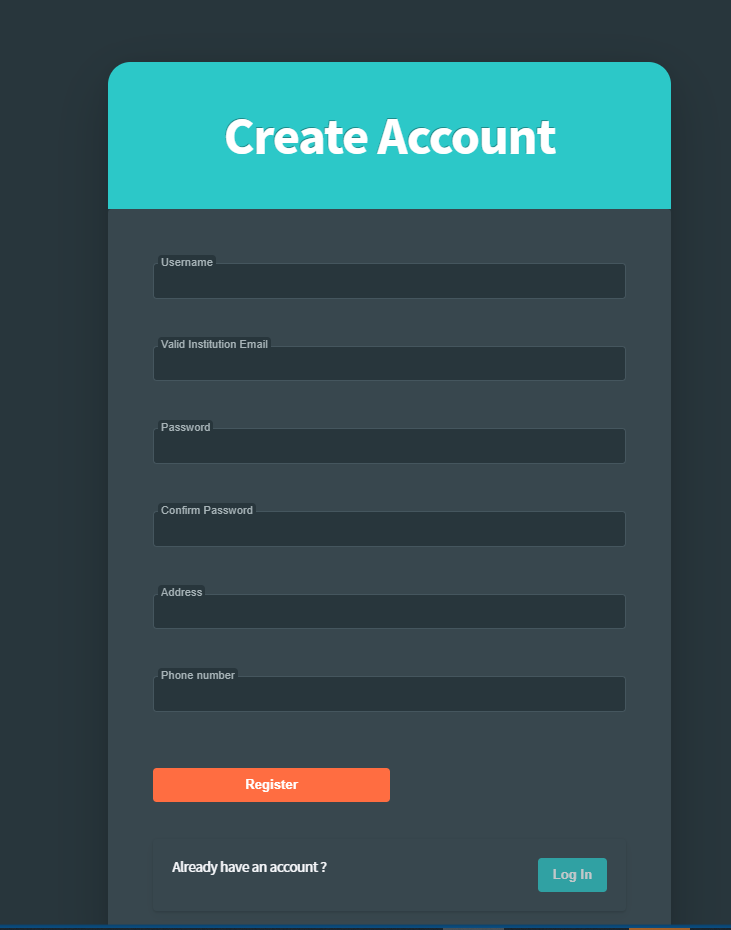
\includegraphics[width=0.5\textwidth]{c1/register.png}
 	\caption{Înregistrarea  pe platformă}
 \end{figure}
 
Această metodă de autentificare se bazează pe o  configurare inițială a unor utilizatori cu drepturi elevate, reprezentanții departamentelor, cărora li se oferă capacitatea de a verifica noii utilizatori care se inregistrează pe platforma utilizând domeniul departamentului în cauză. Fiind pe o parte un mod in plus prin care se limitează accesul utilizatorilor la anumite resurse până când identitatea acestora este confirmată, este pe de altă parte un pas necesar care nu prezintă momentan un sistem de automatizare a verificării identității utilizatorilor, eliminând astfel nevoia unei configurări inițiale a platformei.
	\vspace{0.5 cm}
\begin{figure}[h]
	\centering
	
	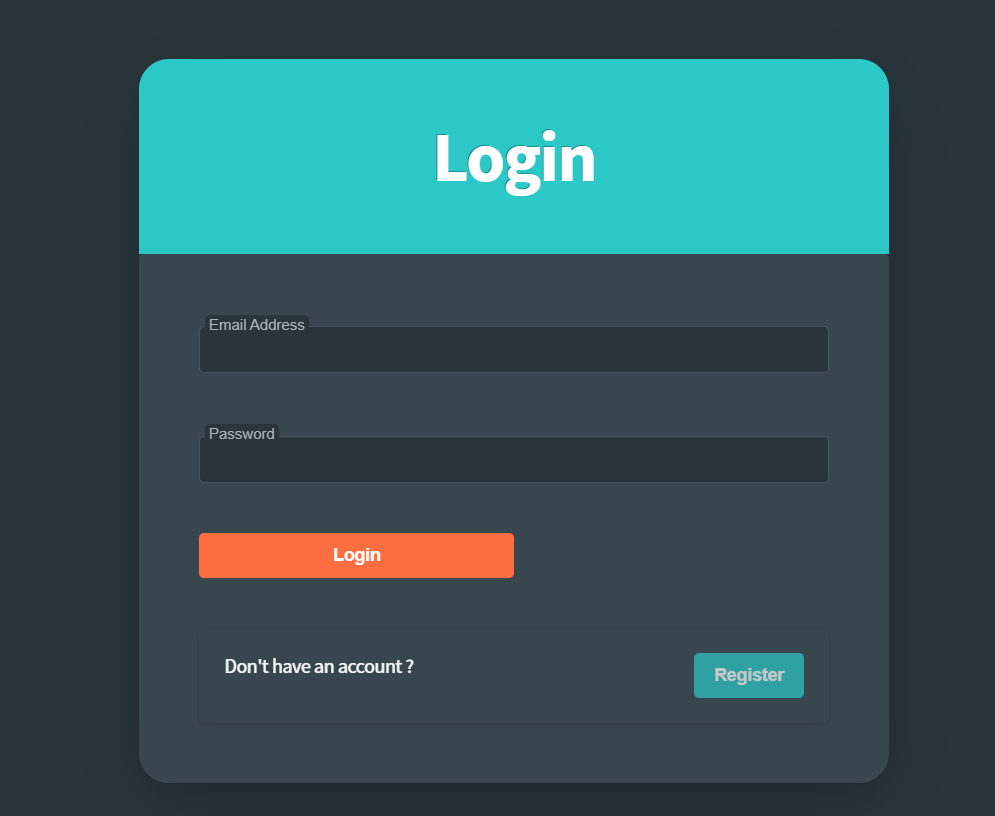
\includegraphics[width=0.5\textwidth]{c1/login.png}
	\caption{Autentificarea pe platformă}
\end{figure}

\subsection{Verificarea acțiunilor utilizatorilor}
În cadrul aplicației, accesul la fiecare entitate este protejat prin implementarea unor liste de acces care definesc permisiunile de scriere și de citire asupra respectivei entități. Acest lucru se asigură că inițial, fiecare utilizator are drept de scriere și de citire doar asupra resurselor create de acesta pe platformă, ulterior acesta având posibilitatea de a acorda sau a primi acces de scriere sau citire asupra altor resurse aflate pe platformă.
	
De asemenea, este implementat și un sistem de roluri care restrictionează și acestea la rândul lor accesul la diferite functionalități ale aplicației, spre exemplu, un utilizator cu rol de reprezentant al unei instituții nu va putea accesa paginile referitoare la crearea sau editarea unei misini de audit.
În plus, pentru o conformitate si pentru o evidență sporită asupra acțiunilor utilizatorilor asupra resurselor de pe platformă este implementat un sistem de auditare al entităților, toate operațiile de creare, modificare și ștergere fiind salvate.

\subsection{Pagina de start}
Pagina de start este locul implicit unde un utilizator este redirecționat atunci când autentificarea sa pe aplicație este cu succes. Aceasta îi prezintă auditorului ultimele modificări la resursele la care are acces, o listă de notificări pe care acesta le-a primit din partea reprezentanților instituțiilor la care auditorul are misiuni de audit în desfășurare cât și diferite butoane de navigare către pagini cheie din aplicație, astfel oferind o interacțiune mai usoară pe platforma AudIT.

\subsection{Gestionarea misinilor de audit public}
În cadrul procesului de audit public, o gestionare eficientă a misiunilor, atât curente cât și din trecut, este esențială pentru o experiență cat mai naturală și intuitivă a utilizatorului pe platformă.

Crearea unei noi misiuni de audit este similară cu crearea unui nou proiect, auditorul specificând numele noii misiuni de audit, instituția respectiv departamentul asupra căruia se realizează noua misiune de audit.

	\vspace{0.5 cm}
\begin{figure}[h]
	\centering
	\begin{minipage}{.5\textwidth}
		\centering
		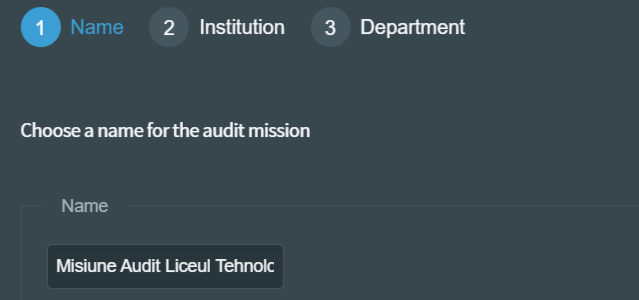
\includegraphics[width=.9\linewidth]{c1/pas1_creare_misiune.png}
		\caption{Stabilirea numelui}
		
	\end{minipage}%
	\begin{minipage}{.5\textwidth}
		\centering
		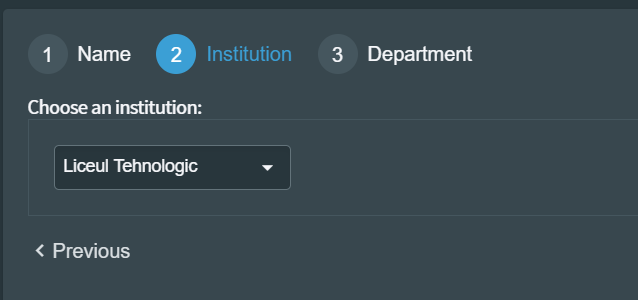
\includegraphics[width=.9\linewidth]{c1/pas2_creare_misiune.png}
		\caption{Selectarea instituției}
	
	\end{minipage}
	\vspace{0.5 cm}

	\centering
	
	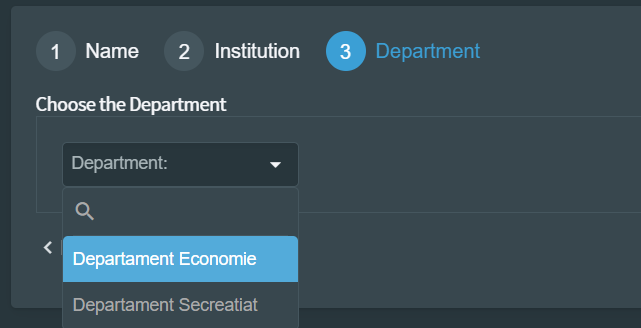
\includegraphics[width=0.5\textwidth]{c1/pas3_creare_misiune.png}
		\vspace{0.5 cm}
	\caption{Selectarea departamentului}
	
	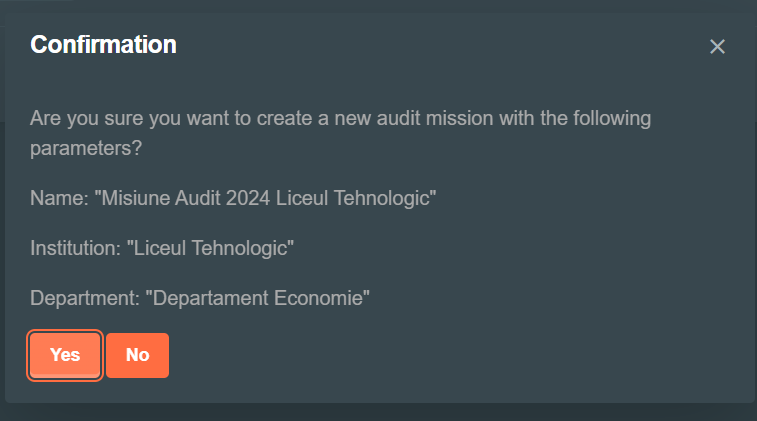
\includegraphics[width=0.5\textwidth]{c1/confirmare_misiune_creata.png}
	\caption{Confirmare creare misiune de audit}
	
\end{figure}


După crearea noii misiuni, auditorul este redirecționat către o pagină în care acesta poate vizualiza intr-un tabel toate misiunile de audit la care acesta are acces, cele create de el, dar și cele la care i-a fost oferit accesul. Afișarea intărilor din tabel este una de tip paginată cu un număr de șapte misiuni pe pagină, astfel încât atenția utilizatorului să fie concentrată doar pe aceste misiuni, în acest fel eliminând posibilitatea de a nu găsi informația pe care acesta o caută datorită unui număr prea mare de linii si informații.
	\vspace{0.5 cm}
\begin{figure}[h]
	\centering
	
	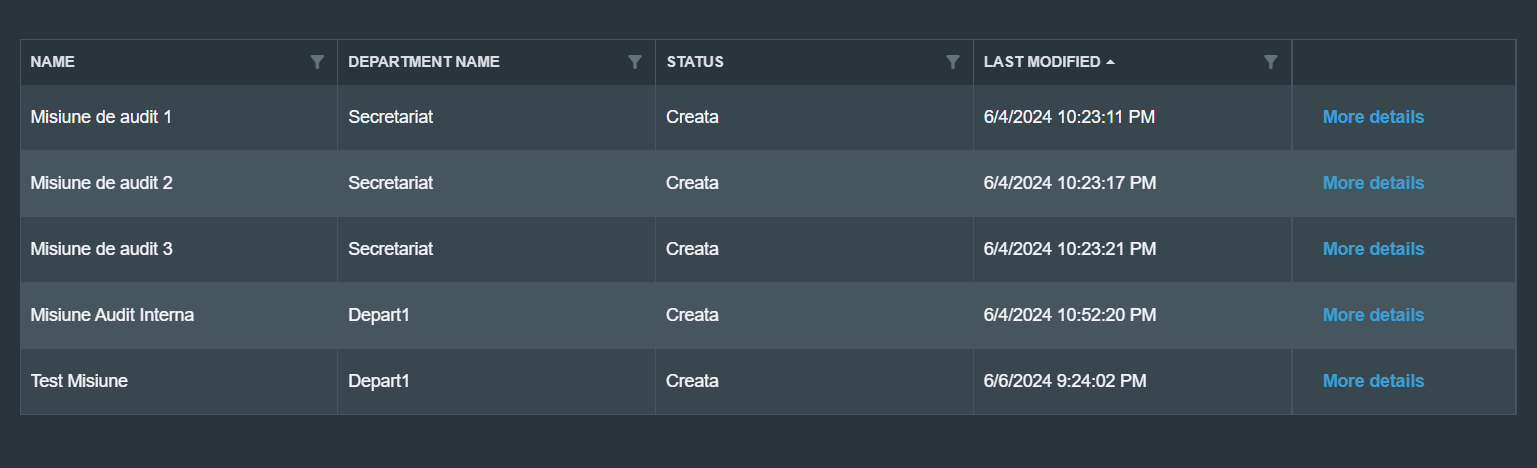
\includegraphics[width=0.8\textwidth]{c1/audit_missions_list.png}
	\caption{Vizualizarea misiunilor de audit}
\end{figure}

De asemenea, informațiile afișate în acest tabel pot fi sortate alfabetic după numele misiunii de audit, după starea în care fiecare dintre acestea se află, după departamentul asupra căruia se desfasoară misiunea  sau după data ultimei modificări a acesteia.

\subsection{Pagina rezumat misiune de audit}

Pagina de rezumat a unei misiuni de audit are ca scop informarea auditorului asupra unei viziuni de ansamblu asupra misiunii de audit respective. Aceasta conține următoarele informații:\\
\begin{itemize}
	
	\item în partea de sus a paginii, auditorului îi este prezentat sub forma unei secvențe de pasi, statusul curent al misiunii, acesta fiind primul lucru pe care privirea utilizatorului il vede;
		
		\begin{figure}[h]
		\centering
		
		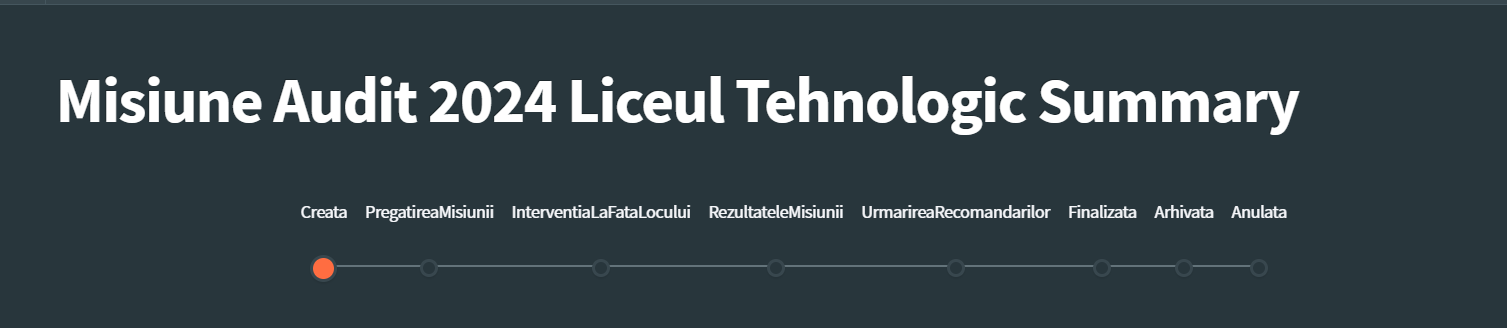
\includegraphics[width=0.9\textwidth]{c1/lant_summary.png}
		\caption{Informații despre statusul misiunii de audit}
	\end{figure}

	\item o scurtă descriere asupra parametrilor misiunii de audit,cum ar fi nume, data ultimii modificări, numele departamentului dar și statusul actual al misiunii. Utilizatorul are opțiunea de a edita acești parametri și a salva modificările aduse;
	
		\vspace{0.5 cm}
	\begin{figure}[h]
		\centering
		
		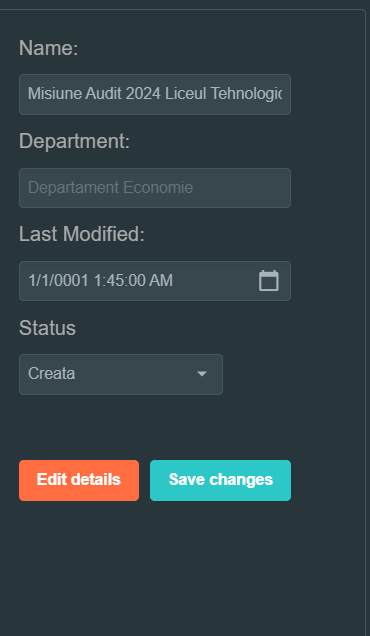
\includegraphics[width=0.5\textwidth]{c1/status_misiune}
		\caption{Informații sumare despre misiunea de audit}
	\end{figure}
	
	\item în partea dreaptă a paginii sunt prezente patru chenare care prezintă cele mai recente modificări și actualizări în materie de : obiective, documente atașate misiunii, fișe de identificare a problemei cât și activități recente asociate misiunii de audit. Utilizatorul are posibilitatea de a naviga apăsând pe numele intrării din lista către pagina dedicată acesteia, sau la apăsarea butonului de 'See more' să fie redirecționat către pagina dedicată tututor entităților de acel fel;
	
	\begin{figure}[h]
		\centering
		
		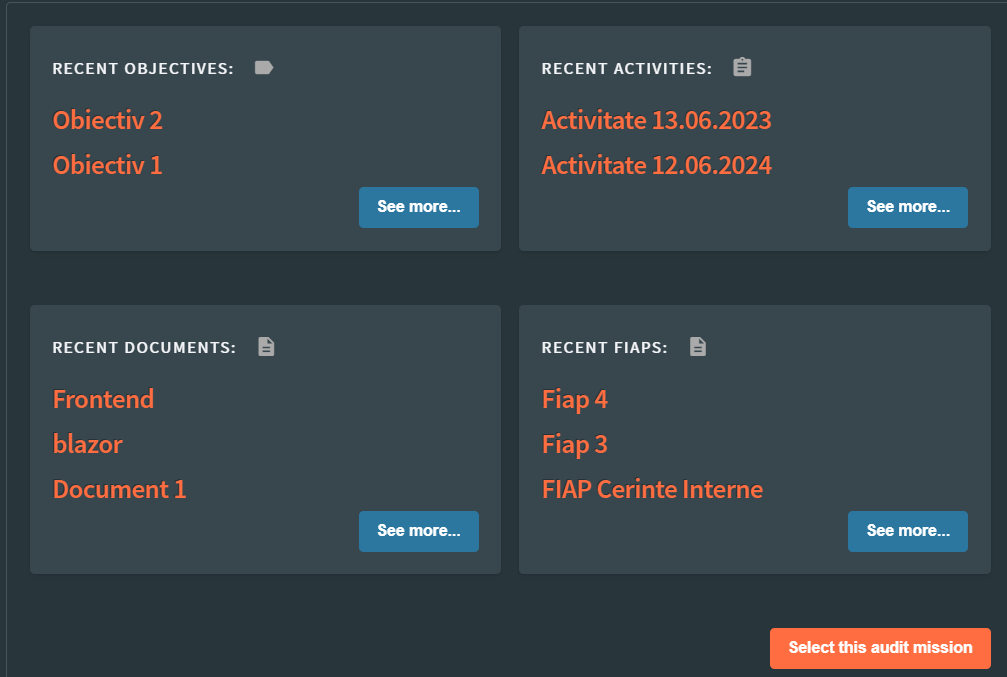
\includegraphics[width=0.7\textwidth]{c1/chenar_recent}
		\caption{Informații sumare despre modificarile recente}
	\end{figure}

	\item în partea dreaptă jos, auditorul are posibilitatea de a selecta misiunea de audit ca fiind misiunea curentă, astfel orice acțiune pe care acesta o sa o facă pe platformă o să ia ca opțiune preselectată misiunea aleasă de acesta.\\
		
	
\end{itemize}


\subsection{Prelucarea pașilor unei misiuni de audit}

Pentru o reproducere cât mai precisă și cooerentă a stagiilor prin care o misiune de audit trece, platforma permite setarea unui status al fiecărei misiuni de audit, astfel auditorul având posibilitatea de a-și marca în detaliu progresul până la momentul curent asupra misiunii de audit. De asemenea, fiecare pas major dintr-o misiune de audit prezintă funcționalități specifice, care vor fi explicate sumar in această subsecțiune.

\subsection*{Pregătirea misiunii de audit}

Pregătirea misiunii de audit este etapa inițială în care auditorul creează misiunea, consultă misiunile anterioare efectuate la același departament, se elaborează un plan de audit, se stabilesc obiectivele, acțiunile specifice fiecărui obiectiv respectiv riscurile specifice fiecărei acțiuni și se întocmesc o serie de documente oficiale, pentru a ține evidența activităților ulterioare pe care auditorul le va realiza în această misiune de audit.

\subsection*{Intervenția la fata locului}

Intervenția la fața locului este o etapă importantă a procesului de audit public, etapă care implică de cele mai multe ori o deplasare in teren unde auditorul efectuează interviuri, realizează eșantioane, analizează riscurile si obiectivele stabilite la pasul anterior și încearcă să înțeleagă într-un mod cât mai corect și obiectiv activitățile desfășurate de departamentul respectiv. Acest pas constă în esență în crearea și completarea a multor documente de tip șablon pe care auditorul le va folosi ulterior în pașii ce urmează pentru a întocmi un raport final.

\subsection*{Rezultatele Misiunii}
După finalizarea pasului anterior, auditorul acum dispune de întreg instrumentalul pentru a întocmi un raport final. Acesta este întocmit pe baza diferitelor întâlniri între auditor și repezentantul instituției, în care se discută aspecte legate de constatările făcute în respectiva misiune de audit. Raportul final cuprinde constatările făcute, recomanandări sub forma 
unor Fișe de Identificare și Analiză a Problemei respectiv cauze și consecințe ale problemelor detectate.

Acest raport este prezentat părților particpante la misiune pentru a le informa asupra rezultatelor misiunii de audit și pentru a ajunge la o înțelegere asupra termenilor de remediere a problemelor pe care aceștia trebuie să le rezolve.

\subsection*{Urmarirea recomandarilor}

Urmărirea recomandărilor este pasul final dintr-o misine de audit în care sunt monitorizate recomandările oferite de către auditor și respectarea termenilor limită de implementare a acestora. Reprezentanții instituțiilor trebuie să ia la cunoștință aceste recomandari și să gasească, ajutați de Fișa de Identificare și Analiză a Problemei corespunzătoare fiecărei recomandari, soluții pentru fiecare chestiune în parte respectând totodată și termenul limită impus de aceasta.


\subsection{Stabilirea obiectivelor de auditat}

Stabilirea obiectivelor de auditat are loc în faza inițială a pasului pregătirii misiunii de audit, pas în care auditorul stabilește obiectivele principale care vor fi auditate în cele ce urmează. Fiecare obiectiv este compus din mai multe acțiuni specifice iar acestea conțin la rândul lor o serie de riscuri identificate. Aceste riscuri identificate de către auditor sunt ierarhizate pe baza unei formule de calcul care ia în considerare probabilitatea acțiunii de a se întâmpla, impactul pe care aceasta îl va avea și riscul final rezultat al inmulțirii celor două.

Platforma web AudIT oferă aceste functionalități utilizatorului, astfel încat acesta să respecte în detaliu toți pașii legislativi ai procedurii de audit public. Auditorul poate forma obiective noi și să le atașeze la misiunea de audit corespunzătoare.\\

\begin{figure}[h]
	\centering
	
	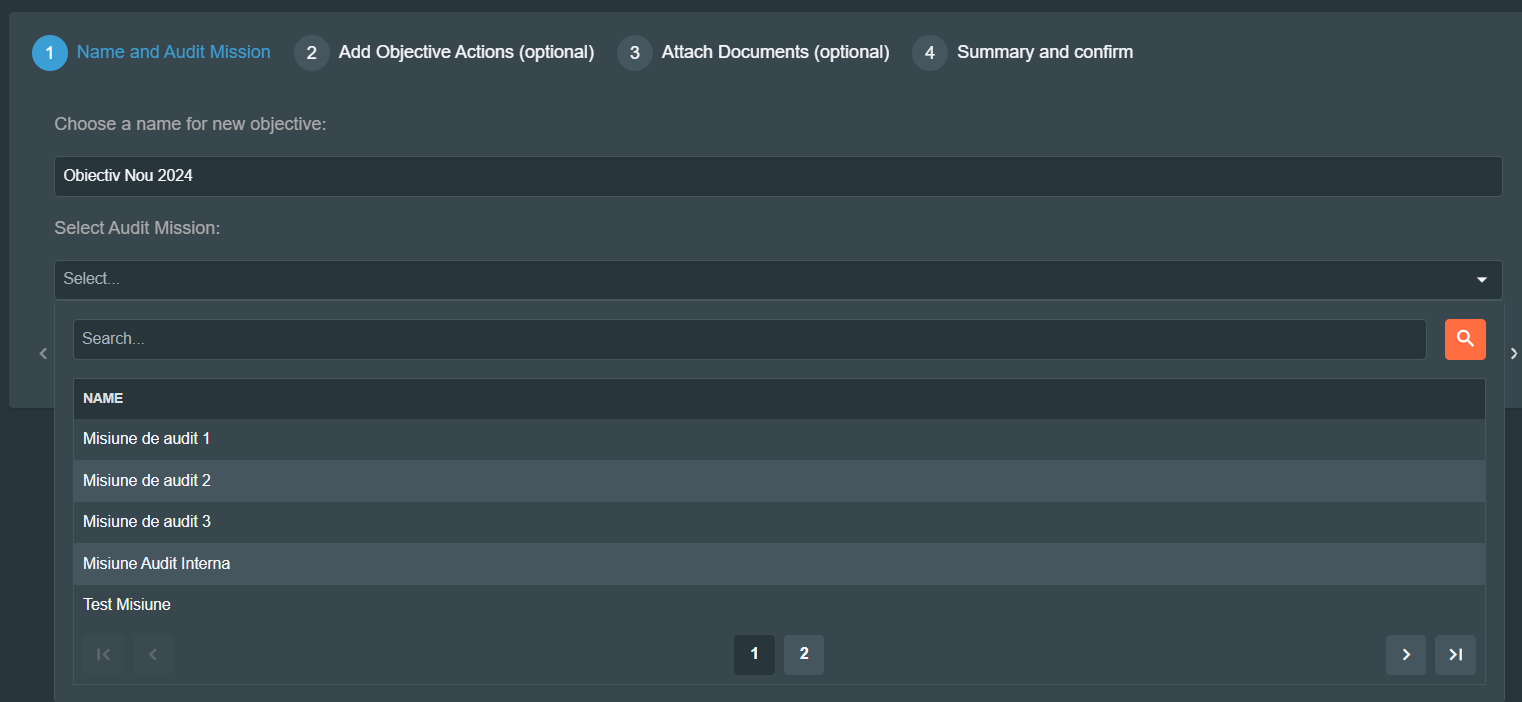
\includegraphics[width=0.8\textwidth]{c1/creare_obiectiv_1}
	\caption{Primul pas în crearea unui nou obiectiv	}
\end{figure}

De asemenea, acesta are posibiliatea de a atașa direct din meniul de creare al unui obiectiv, acțiuni specifice obiectivului respectiv, precum și documente necesare sau ajutătore acțiunii, astfel usurând semnificativ procesul de inventariere prezent la acest pas.

Tot acest proces  de creare a unui nou obiectiv este împărțit pe mai multi pași, astfel încât interacțiunea utilizatorului cu aplicația respectiv cu interfața grafică a acesteia să fie una cât mai naturală și intuitivă.
\vspace{1cm}
\begin{figure}[h]
	\centering
	
	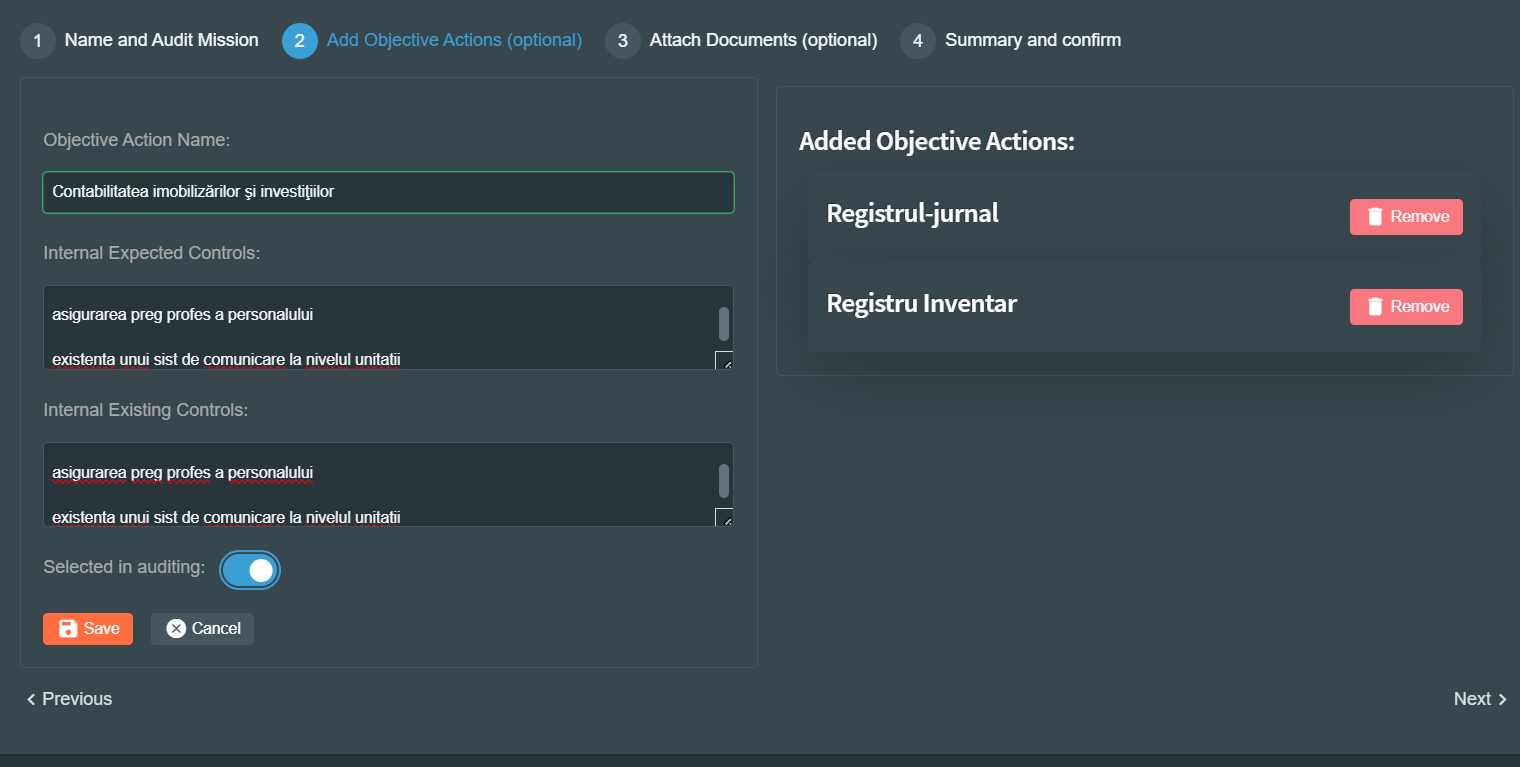
\includegraphics[width=0.9\textwidth]{c1/creare_obiectiv}
	\caption{Atașarea acțiunilor specifice unui obiectiv}
\end{figure}

\subsection{Vizualizarea și accesarea ricurilor din misiuni anterioare}

Stabilirea obiectivelor de auditat, fiind un pas relativ important în procesul de audit public, o identificare cât mai precisă și corectă a riscurilor acțiunilor acestora este crucială pentu o bună desfășurare dar și pentru rezultate optime ale misiunii de audit.

Aplicația oferă auditorului acces la un istoric de misiuni de audit public, în care acesta poate filtra doar misiunile de audit asupra departamentului la care se desfășoară și misiunea de audit curentă, astfel având posibilitatea de analiză a riscurilor ce deja au fost descoperite, ajutându-l 
astfel pe acesta să stabilească noi riscuri relevante, corecte și în conformitate cu situația actuală.

\subsection{Identificarea și evaluarea riscurilor}
Platforma AudIT pune la dispozitia utilizatorului un mecanism de stabilire a riscurilor, aceștia având posibilitatea de a atașa noi riscuri identificate la o acțiune, de a edita valorile riscurilor deja prezente sau de a șterge un risc din tabel în cazul în care acesta nu mai este conform sau o greșeală în definirea acestuia a fost depistată.

Această funcționalitate este implementată prin intermediul unui tabel paginat, fiecare linie afisând informații relevante despre risc, cum ar fi probabilitatea, impactul, scorul final (riscul propriu zis) dar și o scurtă descriere a acestuia.

\vspace{1cm}
\begin{figure}[h]
	\centering
	
	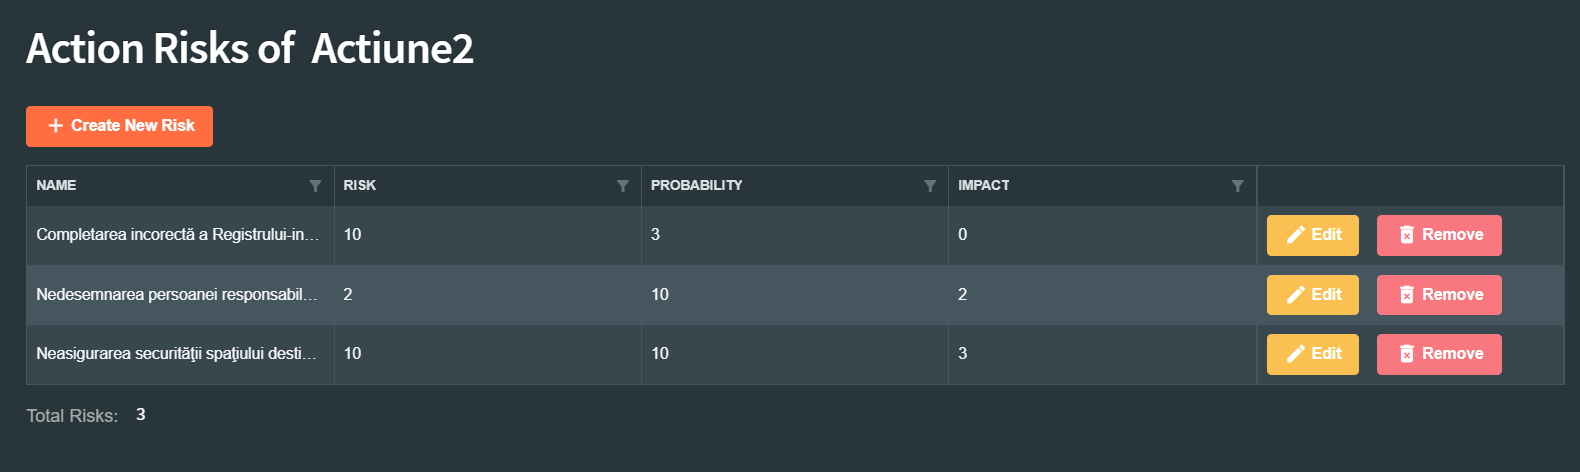
\includegraphics[width=0.9\textwidth]{c1/tabel_riscuri}
	\caption{Informații sumare despre riscurile depistate}
\end{figure}

De asemenea, în partea de jos a tabelului este afișat și numărul total de riscuri atașate acțiunii respective, cât și scorul total al tuturor riscurilor, scor care îl va ajuta ulterior pe auditor in stabilirea selectării sau nu a obiectivul în auditare.

\subsection{Vizualizarea obiectivelor}

Ulterior creării unui nou obiectiv al misiunii de audit, utilizatorul este redirecționat către o pagină în care acesta poate viziona prin intermediul unui tabel toate obiectivele deja stabilite pentru misiunea respectivă de audit într-un format cât mai intuitiv, ușor de folosit și înțeles.

Auditorul poate vizualiza toate acțiunile specifice obiectivului pe care îl analizează, având în plus și informații asupra numelui, data ulitimei modificări/accesări a acesteia, dacă este selectat sau nu în procesul de auditare sau opțiunea de a inspecta toate riscurile identificate până la momentul curent, prin apăsarea butonului 'More details' din dreptul coloanei 'Action Risks Details'.

\vspace{1cm}
\begin{figure}[h]
	\centering
	
	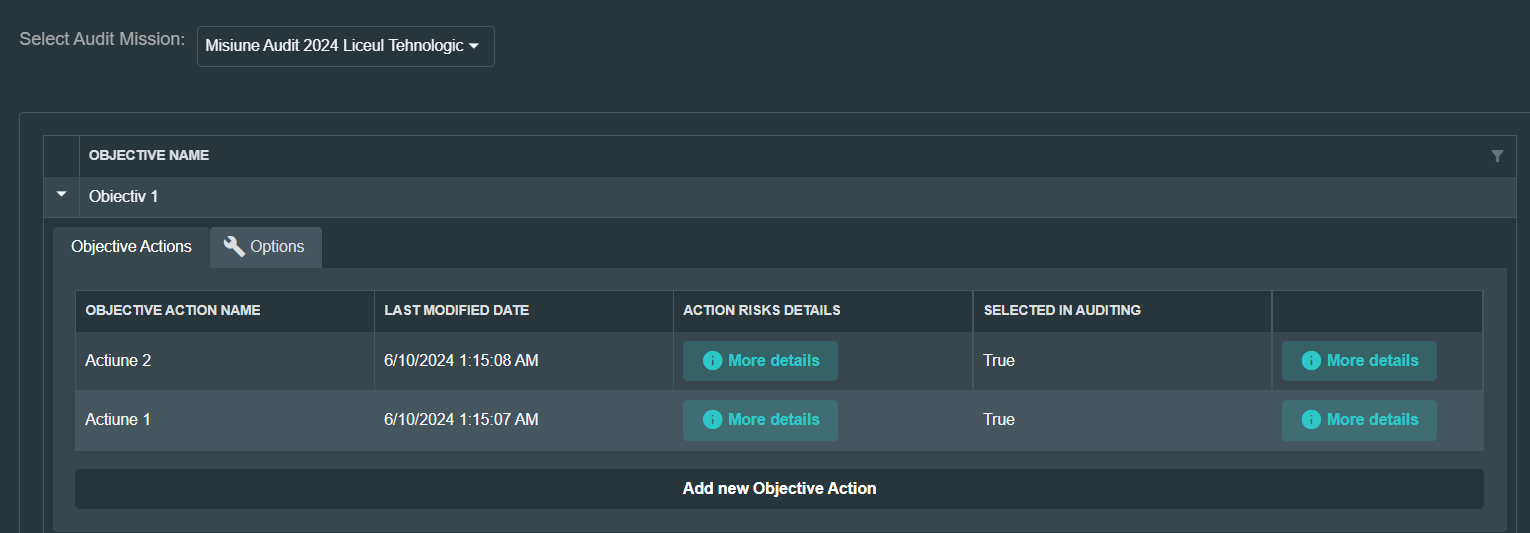
\includegraphics[width=1\textwidth]{c1/tabel_obiective}
	\caption{Informații despre obiectivele misiunii de audit}
\end{figure}



De asemenea, utilizatorul poate naviga prin apăsarea butonului 'More details' din dreptul ultimii coloane către pagina dedicată detaliilor acțiunii, în care acesta poate găsi mai multe amănunte referitoare la acțiunea selectată.


\vspace{1cm}
\begin{figure}[h]
	\centering
	
	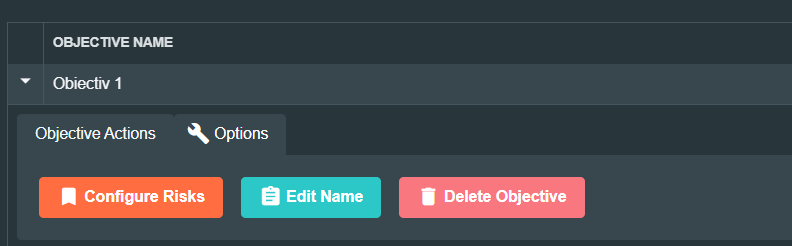
\includegraphics[width=0.9\textwidth]{c1/optiuni_suplimentare}
	\caption{Opțiuni suplimentare gestionare obiectiv}
\end{figure}


\subsection{Pagină detalii actiune}
Pagina oferă auditorului o imagine de ansamblu asupra acțiunii selectate, astfel acesta poate accesa si vizualiza detalii despre acțiune cum ar fi:\\
\begin{itemize}
	\item un scurt rezumat al acesteia care conține numele, dacă este sau nu selectată în procesul de audit, o listă de Controale Interne Așteptate respectiv o listă de Controale Interne Existente;
	
	\item  un tabel în care sunt afișate într-un mod paginat riscurile asociate cu acțiunea respectivă, afisând informații despre impact, probabilitate și scorul riscului;
	
	\item  un tabel care conține informații despre diferite FIAP-uri (Fișă de Identificare și Analiză a Problemei) care sunt asociate cu acțiunea, afișând informații despre numele FIAP-ului, perioada de start și de șfârșit a interacțiunii, problema, cauza si recomandarea oferită de auditor;
	
	\item  un tabel  în care sunt afișate activitățile desfășurate de auditor având ca motiv acțiunea detaliată pe pagină, tabelul prezentând informații despre numele activității, numele departamenutului asupra căruia a avut loc dar și tipul acțiunii;
	
\end{itemize}


\vspace{1cm}
\begin{figure}[h]
	\centering
	
	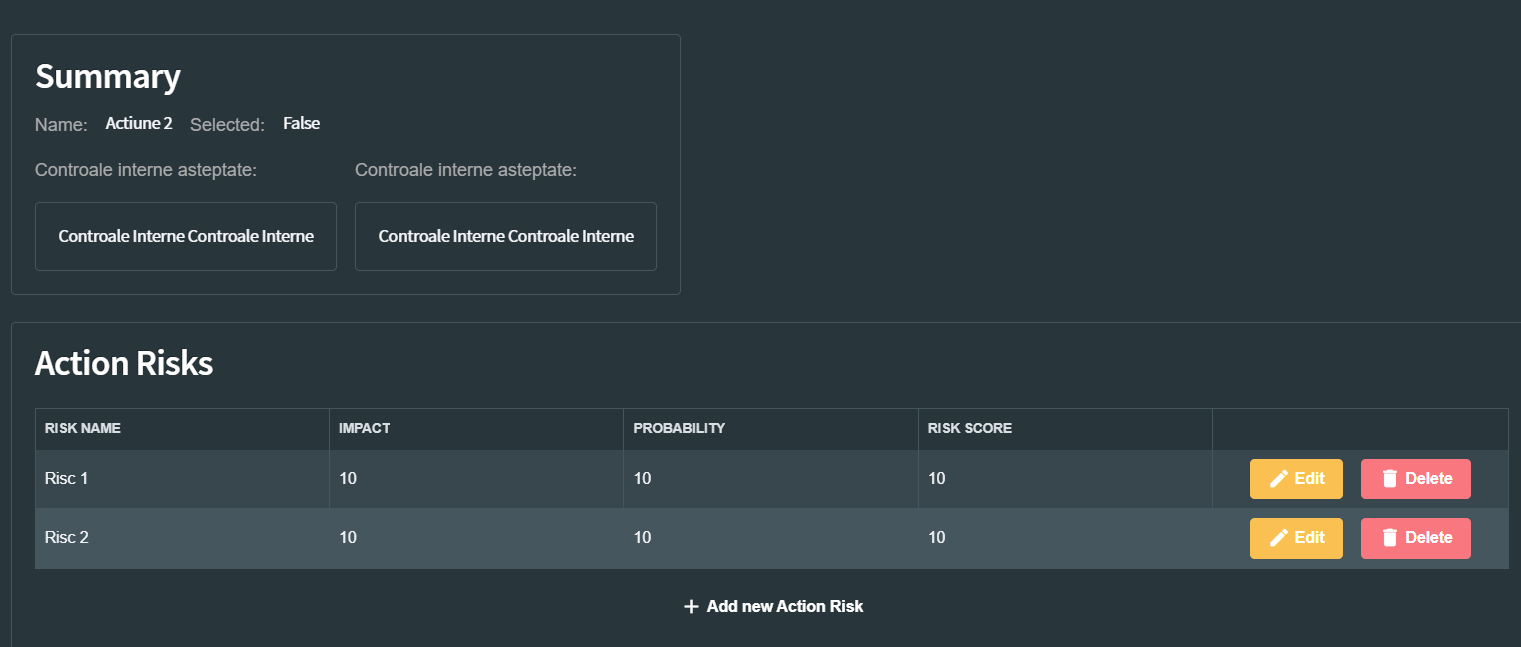
\includegraphics[width=0.9\textwidth]{c1/obiectiv_summary}
	\caption{Informații despre obiectivul selectat}
\end{figure}


De asemenea, în partea de jos a fiecărui tabel, utilzatorul are opțiunea de a adăuga o nouă entitate prin apăsarea butonului 'Add new'. La apăsarea acestuia, se deschide un dialog în care utilizatorul poate completa câmpurile pentru a inițializa o nouă intrare în tabel.

\vspace{1cm}
\begin{figure}[h]
	\centering
	
	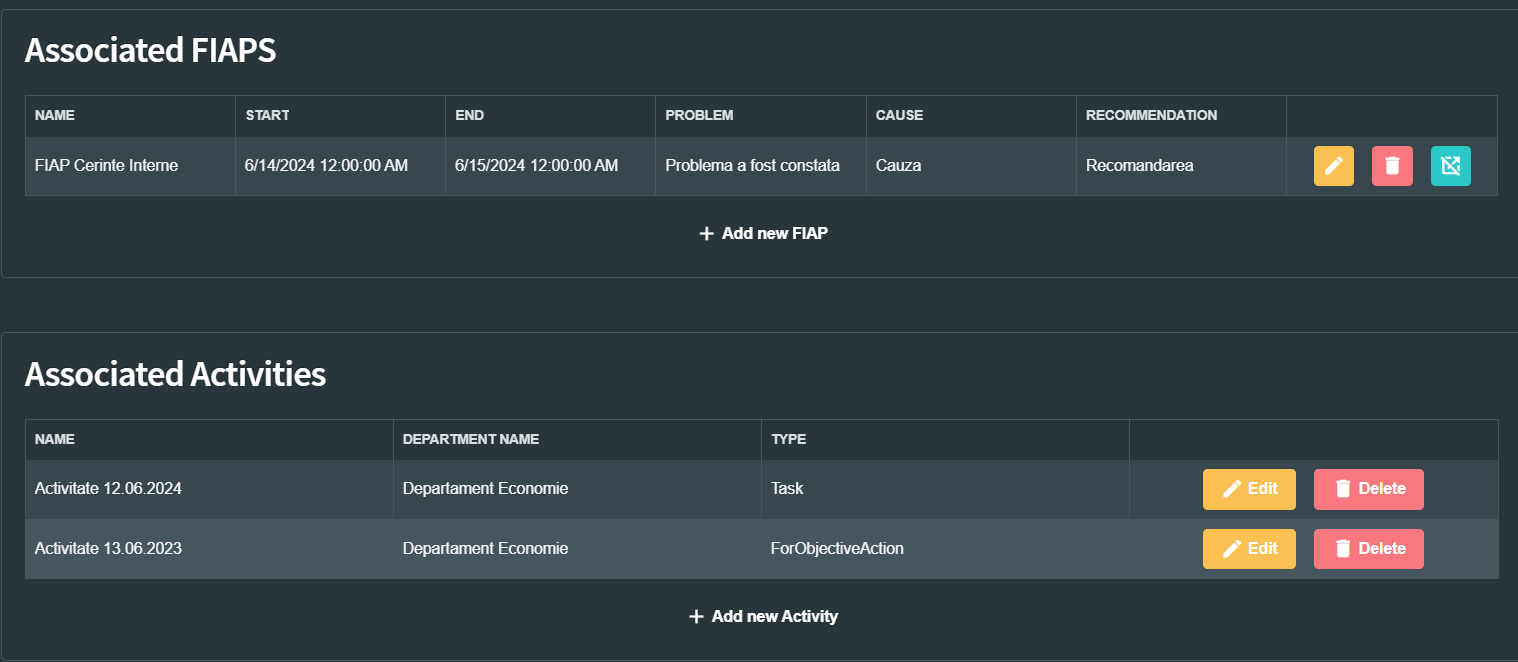
\includegraphics[width=0.9\textwidth]{c1/obiectiv_summary2.png}
	\caption{Informații FIAP și Activități}
\end{figure}


\subsection{Salvarea documentelor necesare pe platformă}

Inventarierea și accesarea documentelor necesare pentru desfășurarea unei misiuni de audit public este o etapă esențială pentru asigurarea transparenței și eficienței procesului de audit public.

Platforma AudIT oferă aceste funcționalități utilizatorilor acesteia, astfel încât atât un auditor cât și membri ai departamentelor auditate care au acces la misiunea de audit, să poată încărca și să salveze pe platformă orice tip de document ce nu depășește o anumită mărime în dimensiune.

La incărcarea unui astfel de document, auditorul are posibilitatea de a alege între tipul documentului încarcat: document standard(un fișier de sine stătător deja completat) sau document șablon(un fișier care necesită completarea acestuia înainte sau ulterior salvării acestuia pe platformă).






 \subsection{Accesarea documentelor necesare pe platformă}
 
 După crearea unui document și salvarea acestuia pe platformă, utilizatorii au opțiunea de a vizualiza documentele elaborate de aceștia respectiv cele la care li s-a oferit accesul.
 
 Afișarea documentelor se face prin intermediul unui tabel, unde sunt afișate informații cum ar fi: numele documentului, tipul documentului, misiunea de audit de care aparține, starea în care acesta se află, ultima dată la care acesta a fost modificat și numele departamentului căruia îi este adresat (în cazul documentelor șablon).
 
 De asemenea, intrările din tabel pot fi filtrate și sortate după diferite criterii, spre exemplu : alfabetic după numele sau tipul documentului, după starea în care acesta se află sau după numele misiunii de audit de care acesta aparține.\\
 
 ---
 
 
 
 
  PIC HERE---\\
 
 
 \subsection{Completarea documentelor tip șablon}
 
	Una dintre sarcinile de bază ale auditorului, dar și un punct nevralgic al sistemului de audit public despre care s-a discutat anterior, îl constituie nevoia de a inventaria și de a completa numeroase documente de tip șablon. Având în vedere faptul că numărul acestor documente este uneori de ordinul zecilor într-o misiune de audit, o funcționalitate care ar permite auditorului să completeze în mediul digital acest tip de documente ar fi bine venită.
	
	Platforma AudIT oferă posibilitatea utilizatorilor să completeze și să editeze direct în aplicație documentele de tip șablon salvate de acestia anterior. Funcționalitatea este implementată prin utilizarea unui simplu editor de text, în care documentul șablon este încărcat, editat, iar la finalizarea procesului, schimbările făcute sunt salvate.
	
	\subsection{Bara de navigare}
	Pentru facilitarea unui acces cât mai ușor la principalele funcționalități ale platformei, utilizatorul se poate folosi de bara de navigare prezentă întotdeauna în partea stângă a aplicației.
	
	Aceasta este împărțită în secțiuni specifice fiecărei entități sau acțiuni, astfel încât se menționează: 
	\begin{itemize}
		\item  secțiunea misiunilor de audit unde regăsim opțiunea de a crea o nouă misiune de audit, de a naviga la misiunea de audit selectată curent, vizualiza lista de misiuni de audit dar și o opțiune de a căuta în fucție de numele misiunii de audit; 
		
		\item secțiunea obiectivelor în care există opțiunile de creare a unui nou obiectiv, navigare către pagina tututor obiectivelor, crearea a noi acțiuni specifice unui obiectiv dar și posibilitatea de a căuta un obiectiv al misiunii de audit curente în funcție de numele acestuia;
		
		\item secțiunea recomandărilor unde auditorul poate adăuga o nouă recomandare dar și vizualiza recomandările deja existente;
		
		\item secțiunea documentelor unde similar, merg adăugate noi documente și vizualiza documente deja existente pe platformă;
		
		\item secțiunea activităților unde utilizatorul poate consemna activități noi desfășurate sau naviga spre cele existente deja;
		
		\item secțiunea dedicată exportării, unde auditorul poate naviga spre diferite pagini de convertire a obiectivelor, acțiunilor și a riscurilor în diferite formate dar și autocompletare a unor documente oficiale de tip șablon, cum ar fi Fișe de Identificare a Problemei sau Raport de Evaluarea a Riscurilor;
		
		\item secțiunea de control al accesului, unde auditorul sau reprezentanții instituțiilor audidate pot consulta resursele la care au acces de scriere sau citire respectiv a oferi acces altor utilizatori la resurse personale;
		
		\item secțiunea de configurare, unde un utilizator cu drepturi elevate poate configura instituțiile respectiv departamentele înregistrate pe platformă, adăugând, editând sau eliminând instanțe dintre acestea.
		
		
		
		

	\end{itemize}
\newpage
   De asemenea, bara de navigare se actualizează în funcție de statusul de autentificare și de rolul pe care utilizatorul îl are.
   \begin{figure}[h]
   	\centering
   	\begin{minipage}{.5\textwidth}
   		\centering
   		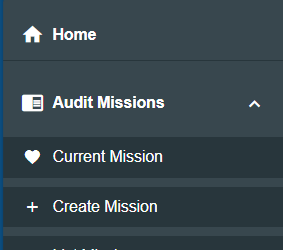
\includegraphics[width=.9\linewidth]{c1/navbar_logat}
   		\caption{Utilizator autentificat}
   		
   	\end{minipage}%
   	\begin{minipage}{.5\textwidth}
   		\centering
   		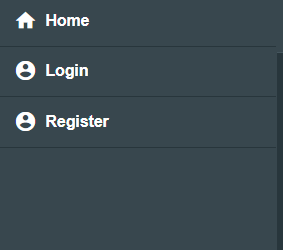
\includegraphics[width=.9\linewidth]{c1/navbar_nelogat.png}
   		\caption{Utilizator neautentificat}
   		
   	\end{minipage}
   	
   	
   \end{figure}

	\subsection{Gestionarea accesului la resurse partajate}
	
	 O componentă cheie in desfășurarea corectă a unei misiuni de audit este colaborarea între părțile participante la misiunea de audit.
	 
		Funcționalitatea de acordare a accesului la resurse, contribuie la o colaborare cât mai strânsă între membrii partipanți la misiunea de audit, astfel un auditor poate acorda acces de scriere sau citire la diferite resurse create de acesta.
		
		În plus, o listă completă a accesului primit sau oferit se poate vizualiza de către utilizator pe o pagină dedicată, unde sub forma unui tabel sunt prezentate informații specifice cum ar fi numele și tipul resursei și email-ul utilizatorului căruia i s-a oferit  acces.
		
	\subsection{Gestionarea activităților desfășurate}
	 Prin această funcționalitate, auditorul poate consemna orice sarcină pe care acesta o efectuează pe platformă prin intermediul unei activități. Aceasta cuprinde informații referitoare la acțiunea asupra căreia s-a efectuat o activitate, departamentul asociat dar si tipul activității care poate fi asociat unei misiuni, unei acțiuni sau pur și simplu o sarcină administrativă.
	 
	 De asemenea , toate activitățile consemnate într-o misiune de audit, pot fi vizualizate de către auditor într-o pagină dedicată, acestea fiind afisate prin intermediul unui tabel care oferă informații referitoare la numele acesteia, tipul acțiunii sau departamentul asupra căruia s-a realizat respectiva sarcină.
	 
	
	\subsection{Profilul personal}
	Pagina profilul personal este locul unde utilizatorul poate sa își verifice informațiile personale care sunt disponibile pe platformă având posibilitatea de a le edita. Informațiile cuprind detalii de contact, cum ar fi adresa de email principală, cea secundară, număr de telefon al instituției, număr de telefon personal, adresa fizică de contact respectiv dacă acesta este verificat sau nu.
 
	
	\subsection{Sistemul de notificări}
		Funcționalitatea permite vizualizarea notificărilor în ceea ce privește crearea de noi resurse, primirea accesului la o anumită resursă sau notificări în ceea ce privește actualizarea sau implementarea unor soluții la recomandările impuse de auditor din partea reprezentanților instituției asupra căreia are loc misiunea de audit.


	\section{Solutii similare}
	Soluția descrisă nu este o idee unică, dar este esențial să studiem și să întelegem modul în care soluțiile similare abordeaza această problemă, având astfel posibiliatea să identificăm puncte forte cât și puncte slabe ale aplicației ce merg ulterior imbunătățite, inovând acolo unde este posibil.
	
	În secțiunea următoare o să fie prezentate câteva soluții similare adresate problemei de digitalizare în domeniul auditului public și o să fie analizate functionalitătile inedite ale acestora. 
	
	\subsection*{Audit Pro}
	
	Audit Pro este o aplicație dezvoltată în special pentru sistemul de operare Windows și care încearcă să ofere un mediu de lucru eficient auditorilor.
	
	Soluția oferită este una care se bazează pe achiziționarea acesteia contra unui pret, oferind în pachet si o configurare inițială a instituțiilor si membrilor din departamentul de audit.
	
	Aceasta oferă funcționalități similare cu soluția descrisă în acest document, dar printre care se evidențiază:
	 
	\begin{itemize}
		\item accesul la un calendar unde auditorul poate vizualiza evenimentele importante ce vor avea sau au avut loc, având de asemenea posibilitatea de a adăuga noi evenimente în acesta;
		
		\item o pagină dedicată analizei costurilor desfășurării anumitor activități specifice unei misiuni de audit: costuri de deplasare, diurne etc;
		
		\item un meniu de ajutor unde utilizatorul poate accesa informații ajutătoare în vederea utilizării anumitor funcționalități din aplicație;
		
	\end{itemize}
	
	\vspace{1cm}
	\begin{figure}[h]
		\centering
		
		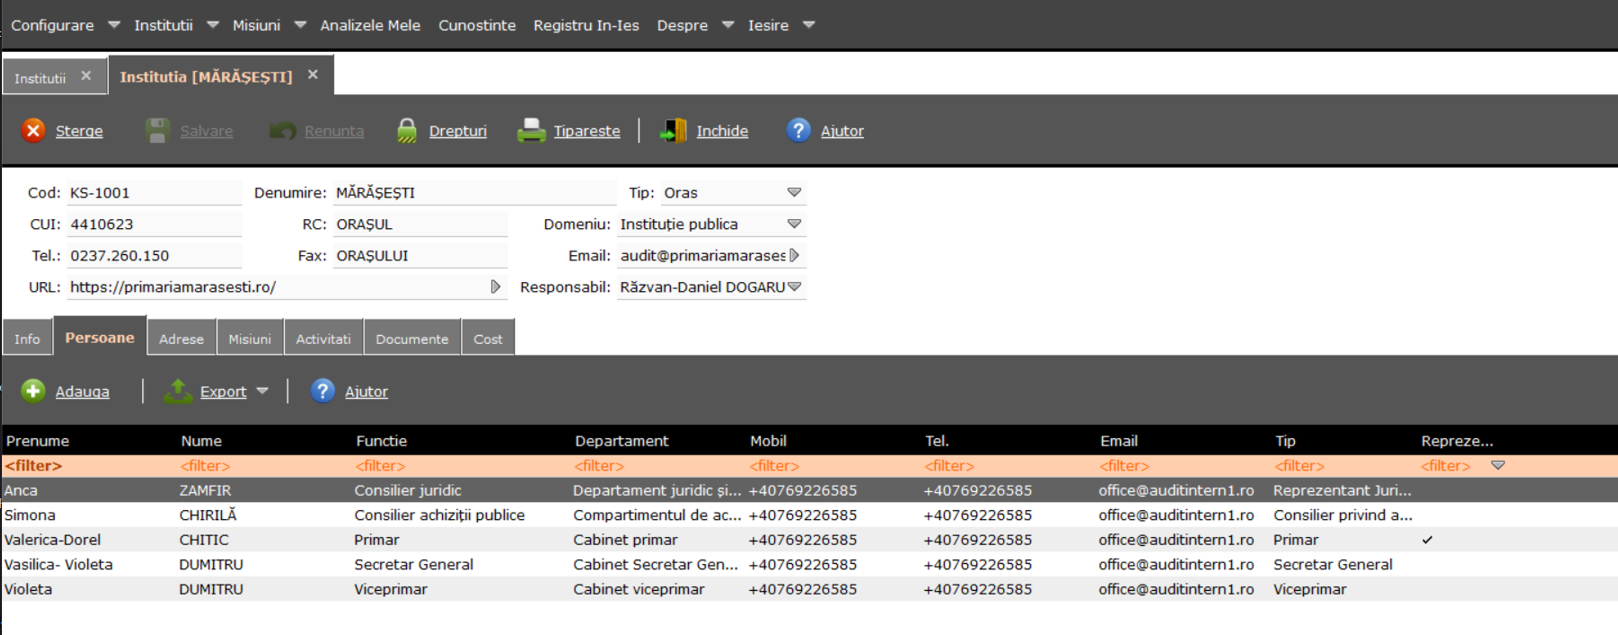
\includegraphics[width=0.9\textwidth]{c1/auditpro1}
		\caption{Tabel din aplicația Audit Pro}
	\end{figure}
	
	
	
Pe de altă parte, soluția descrisă prezintă și anumite dezavantaje care constau în modul în care aceasta a fost implementată, unul dintre acestea fiind limitarea strict la utilizarea acesteia numai pe sistemul de operare Windows, mărginind în acest mod alte sisteme de operare prezente.
De asemenea, din punctul meu de vedere, aspectul grafic și interfața pe care aceasta solutie o prezintă nu este una foarte intuitivă si poate induce în eroare utilizatorii în anumite situații.
\vspace{1cm}
\begin{figure}[h]
	\centering
	
	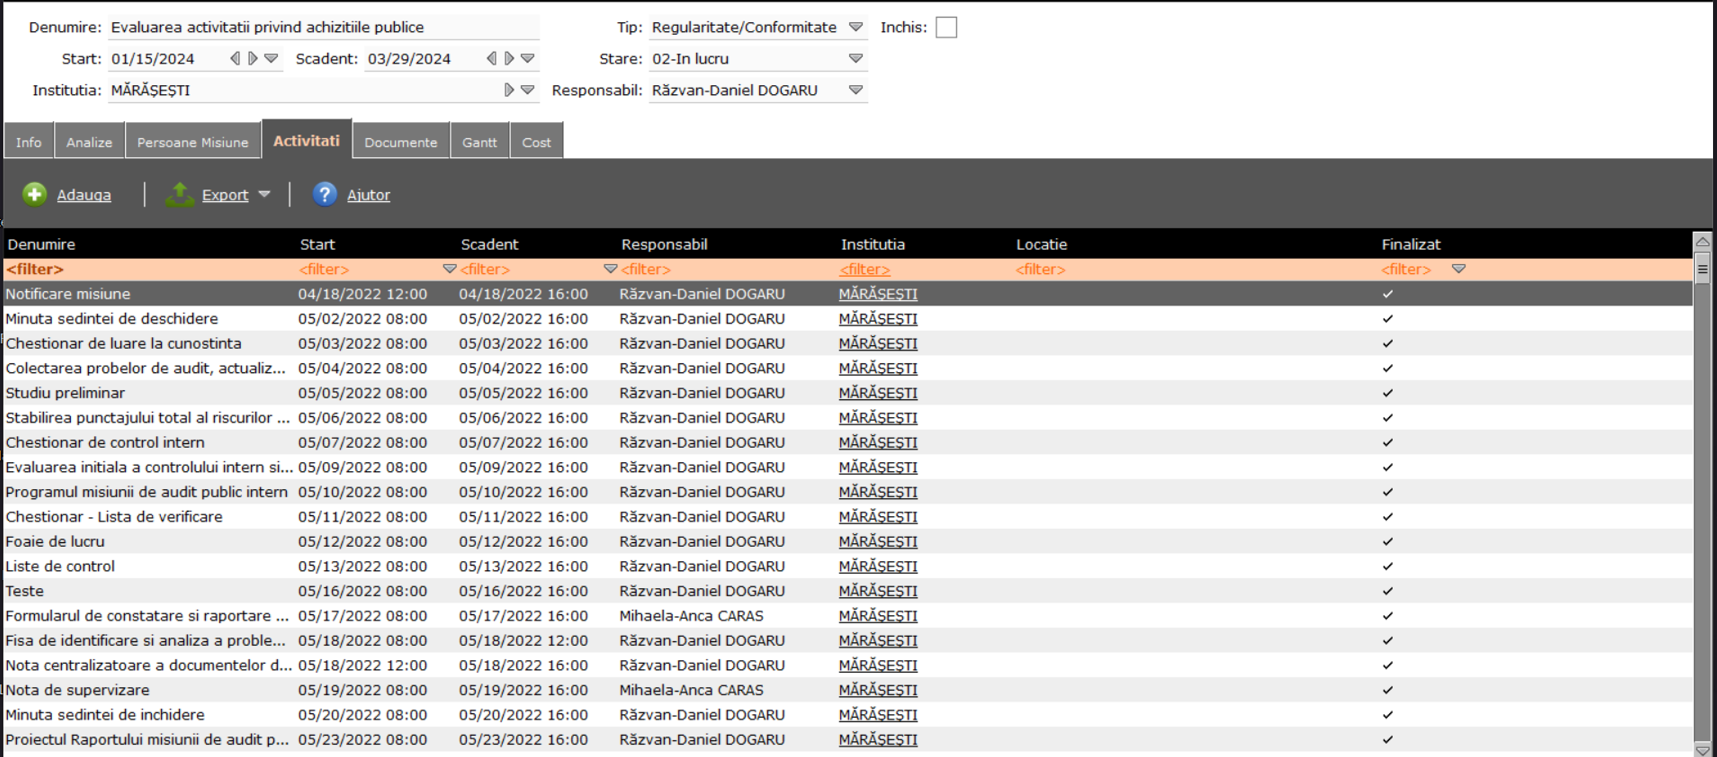
\includegraphics[width=0.9\textwidth]{c1/auditpro2}
	\caption{Tabel din aplicația Audit Pro}
\end{figure}

	\newpage
	\subsection*{Site Audit Pro }
	
	Chiar dacă numele este similar cu soluția prezentată anterior, este vorba despre un alt proiect, de aceasta dată o platforma web cu suport și pentru aplicație mobilă care prezintă soluții pentru auditul în sectorul privat, cel al companiilor.
	
	Din informațiile prezente pe pagina  lor de prezentare, se poate trage concluzia că această soluție este una ajunsă la maturitate, primind constant actualizări în ceea ce privește funcționalitățile oferite de aceasta.
	 
	Dintre numeroasele facilități pe care această soluție le oferă, cele mai importante și cu un impact mai mare ar putea fi:
	\begin{itemize}
		\item posibilitatea de a lucra in mediul \textit{offline} pe platforma mobilă, informațiile fiind actualizate cu server-ul principal în momentul în care există o conexiune la internet;
		
		\item sincronizarea proiectelor pe toate dispozitivele (Web, Android si IOS) astfel încât toate informațiile să fie actualizate în timp real;
		
		\item organizarea proiectelor și resurselor în directoare, facilitând astfel o navigare mai eficientă ;
	\end{itemize}
	\begin{figure}[h]
		\centering
		
		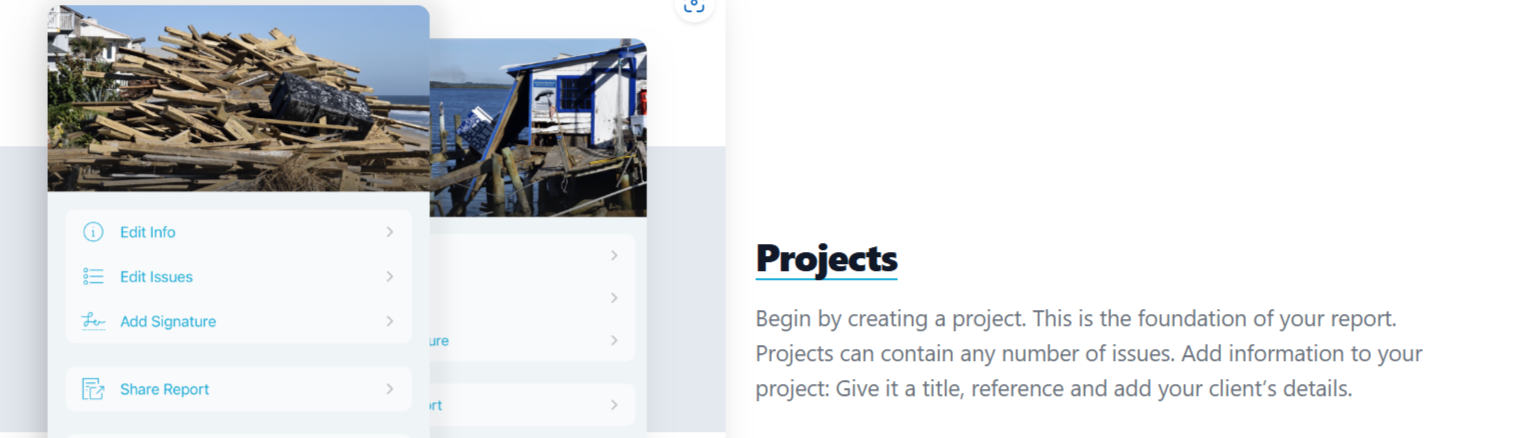
\includegraphics[width=0.6\textwidth]{c1/auditpro3}
		\caption{Tabel din platforma Site Audit Pro}
	\end{figure}
	
	Cu toate acestea, un dezavantaj pe care această soluție îl oferă este acela că procedurile pe care aceasta este construită, nu se mulează și nu corespund în cea mai mare parte cu cele din sistemul de audit public din România, utilizatorii trebuind astfel să se adapteze și să încerce pe cât posibil să personalizeze și să modifice funcționalitățile oferite de aceștia.
	
	
	
	
